\chapter{Обзор аналогов}
\section{SpeedTree}
\subsection{История}
\emph{SpeedTree} - комплекс программных продуктов, разрабатываемый компанией Interactive Data Visualisation. 

Первая версия SpeedTree называлась SpeedTreeCAD и была создана IDV в 2000 году для использования в симуляторе гольфа. Позже CAD был преобразован в плагин для 3D Studio Max (ныне Autodesk 3ds Max) под названием SpeedTreeMax. 

В конце 2002 года IDV выпустила SpeedTreeRT - SDK для рендеринга деревьев в реальном времени. SpeedTreeRT поддерживал несколько уровней детализации, эффект ветра и различные уровни освещения. Также был разработан SpeedTreeMAYA - аналогичный SpeedTreeMax плагин для Maya. 

В 2009 году разработка этих плагинов была завершена, и им на смену пришёл SpeedTree 5. В его состав вошли три компонента: редактор SpeedTree Modeler, SpeedTreeSDK и SpeedTree Compiler, предназначенный для подготовки файлов SpeedTree к рендерингу в реальном времени. 

Пример дерева, созданного при помощи SpeedTree, представлен на рисунке ~\ref{fig:speedtree}. Как видно по рисунку, результирующие модели фотореалистичны и подходят для использования в высокобюджетных фильмах. 

\subsection{Состав}
В настоящее время SpeedTree включает в себя следующие программные комплекты:
\subsubsection{SpeedTree Cinema}
\emph{SpeedTree Cinema} - комплект программного обеспечения, предназначенный для использования в кинематографе. Он был выпущен в 2009 и с тех пор широко используется для генерации деревьев в фильмах, начиная с ``Аватара'' Джеймса Кэмерона. SpeedTree Cinema генерирует полигональные сетки и текстуры высокого разрешения для различных редакторов трёхмерной графики.

\subsubsection{SpeedTree Studio}
\emph{SpeedTree Studio} является бюджетной версией SpeedTree Cinema. Он включает в себя подмножество возможностей этого комплекта.

\subsubsection{SpeedTree Architect}
\emph{SpeedTree Architect} предназначен для экспорта моделей в CAD, такие, как Maya и Autodesk 3ds Max.

\subsubsection{SpeedTree for Games}
\emph{SpeedTree for Games} - издание, предназначенное для разработки игр. Оно включает в себя Modeler, Compiler и SDK и может быть интегрировано в любой игровой движок. Сгенерированные полигональные сетки отличаются большей оптимизацией по сравнению с другими изданиями SpeedTree.

\subsubsection{SpeedTree Subscription Edition}
\emph{SpeedTree Subscription Edition} - бюджетное решение, рассчитанное на независимых разработчиков игр. Подписка на этот продукт даёт доступ к редактору и генерации деревьев и растений. Полученные модели могут быть использованы только в Unity или Unreal Engine, в зависимости от приобретённой лицензии. Также за дополнительную плату можно приобрести комплекты готовых моделей из библиотеки.

\begin{figure}[h]
    \centering
    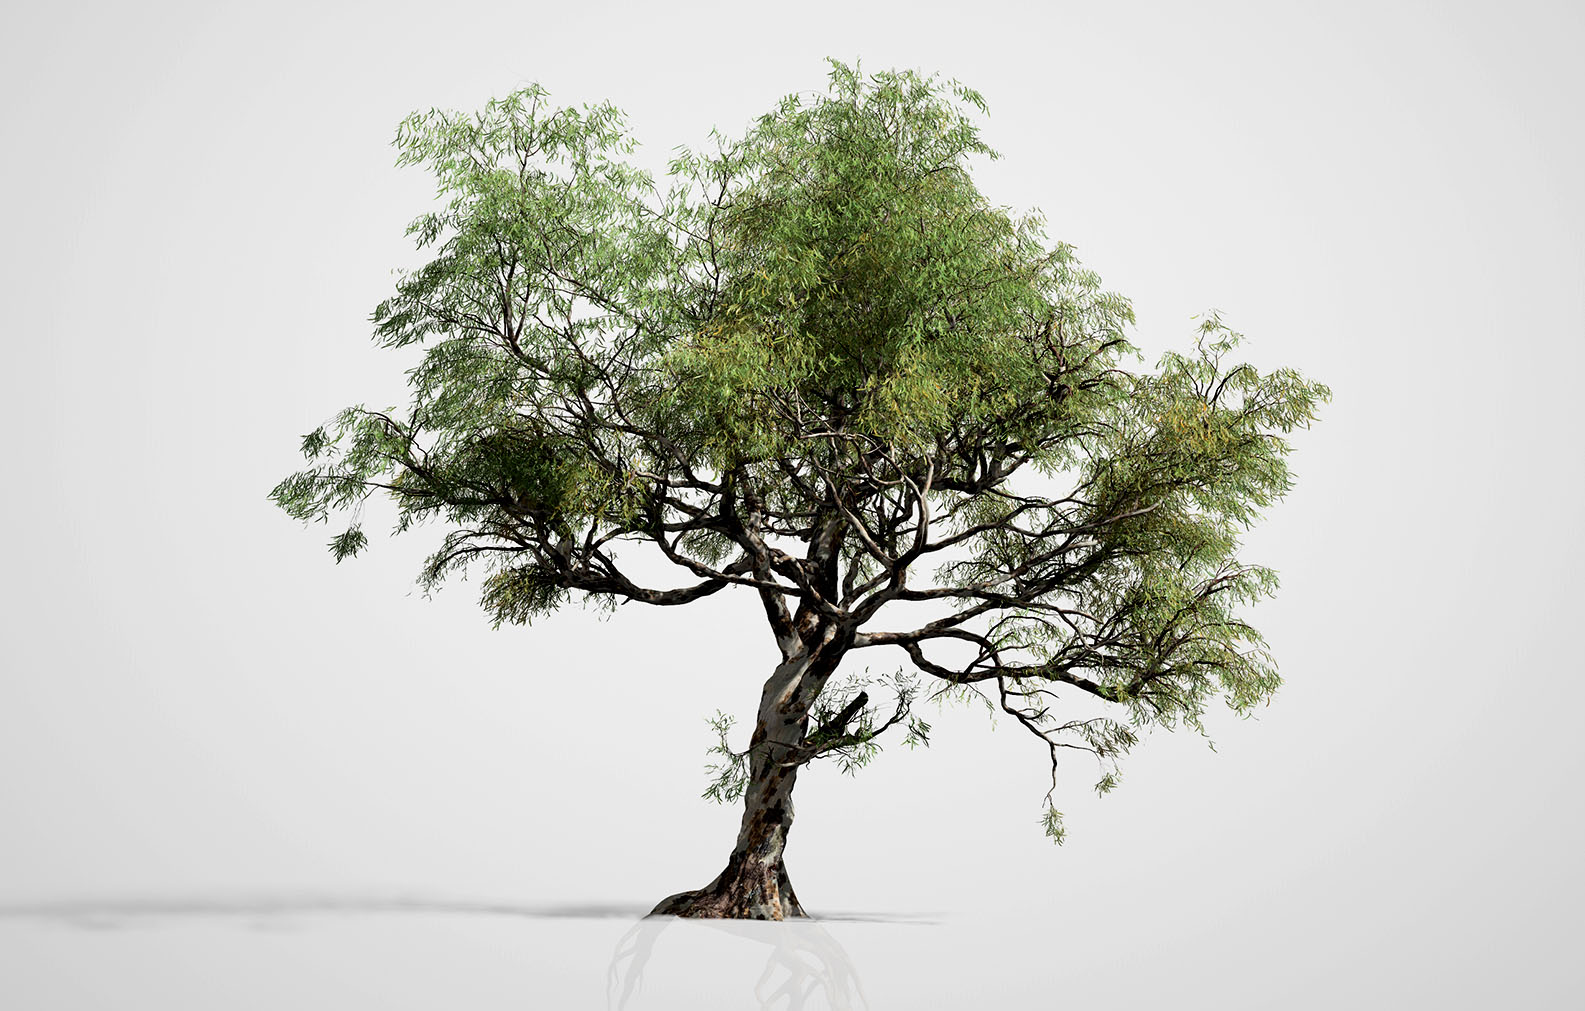
\includegraphics[width=0.8\textwidth]{speedtree}
    \caption{Пример дерева, сгенерированного при помощи SpeedTree.}
    \label{fig:speedtree}
\end{figure}

\section{TreeIt}
\emph{TreeIt} - бесплатное программное обеспечение для генерации растительности, разработанное Evolved Software для Microsoft Windows. TreeIt позволяет создавать модели растений различных видов, включая не только деревья, но также кактусы и цветы.

Поддерживается экспорт в форматы dbo, obj, fbx и x. Присутствует возможность регуляции уровня детализации. Все модели, сгенерированные при помощи TreeIt, абсолютно бесплатны для использования в любых проектах.

В редактор TreeIt входит встроенный набор текстур, что упрощает создание моделей. Также на официальном сайте TreeIt\cite{treeit} можно скачать библиотеку заранее настроенных шаблонов растений. 

На рисунке ~\ref{fig:treeit} показана кокосовая пальма, созданная при помощи TreeIt. 

\begin{figure}[h]
    \centering
    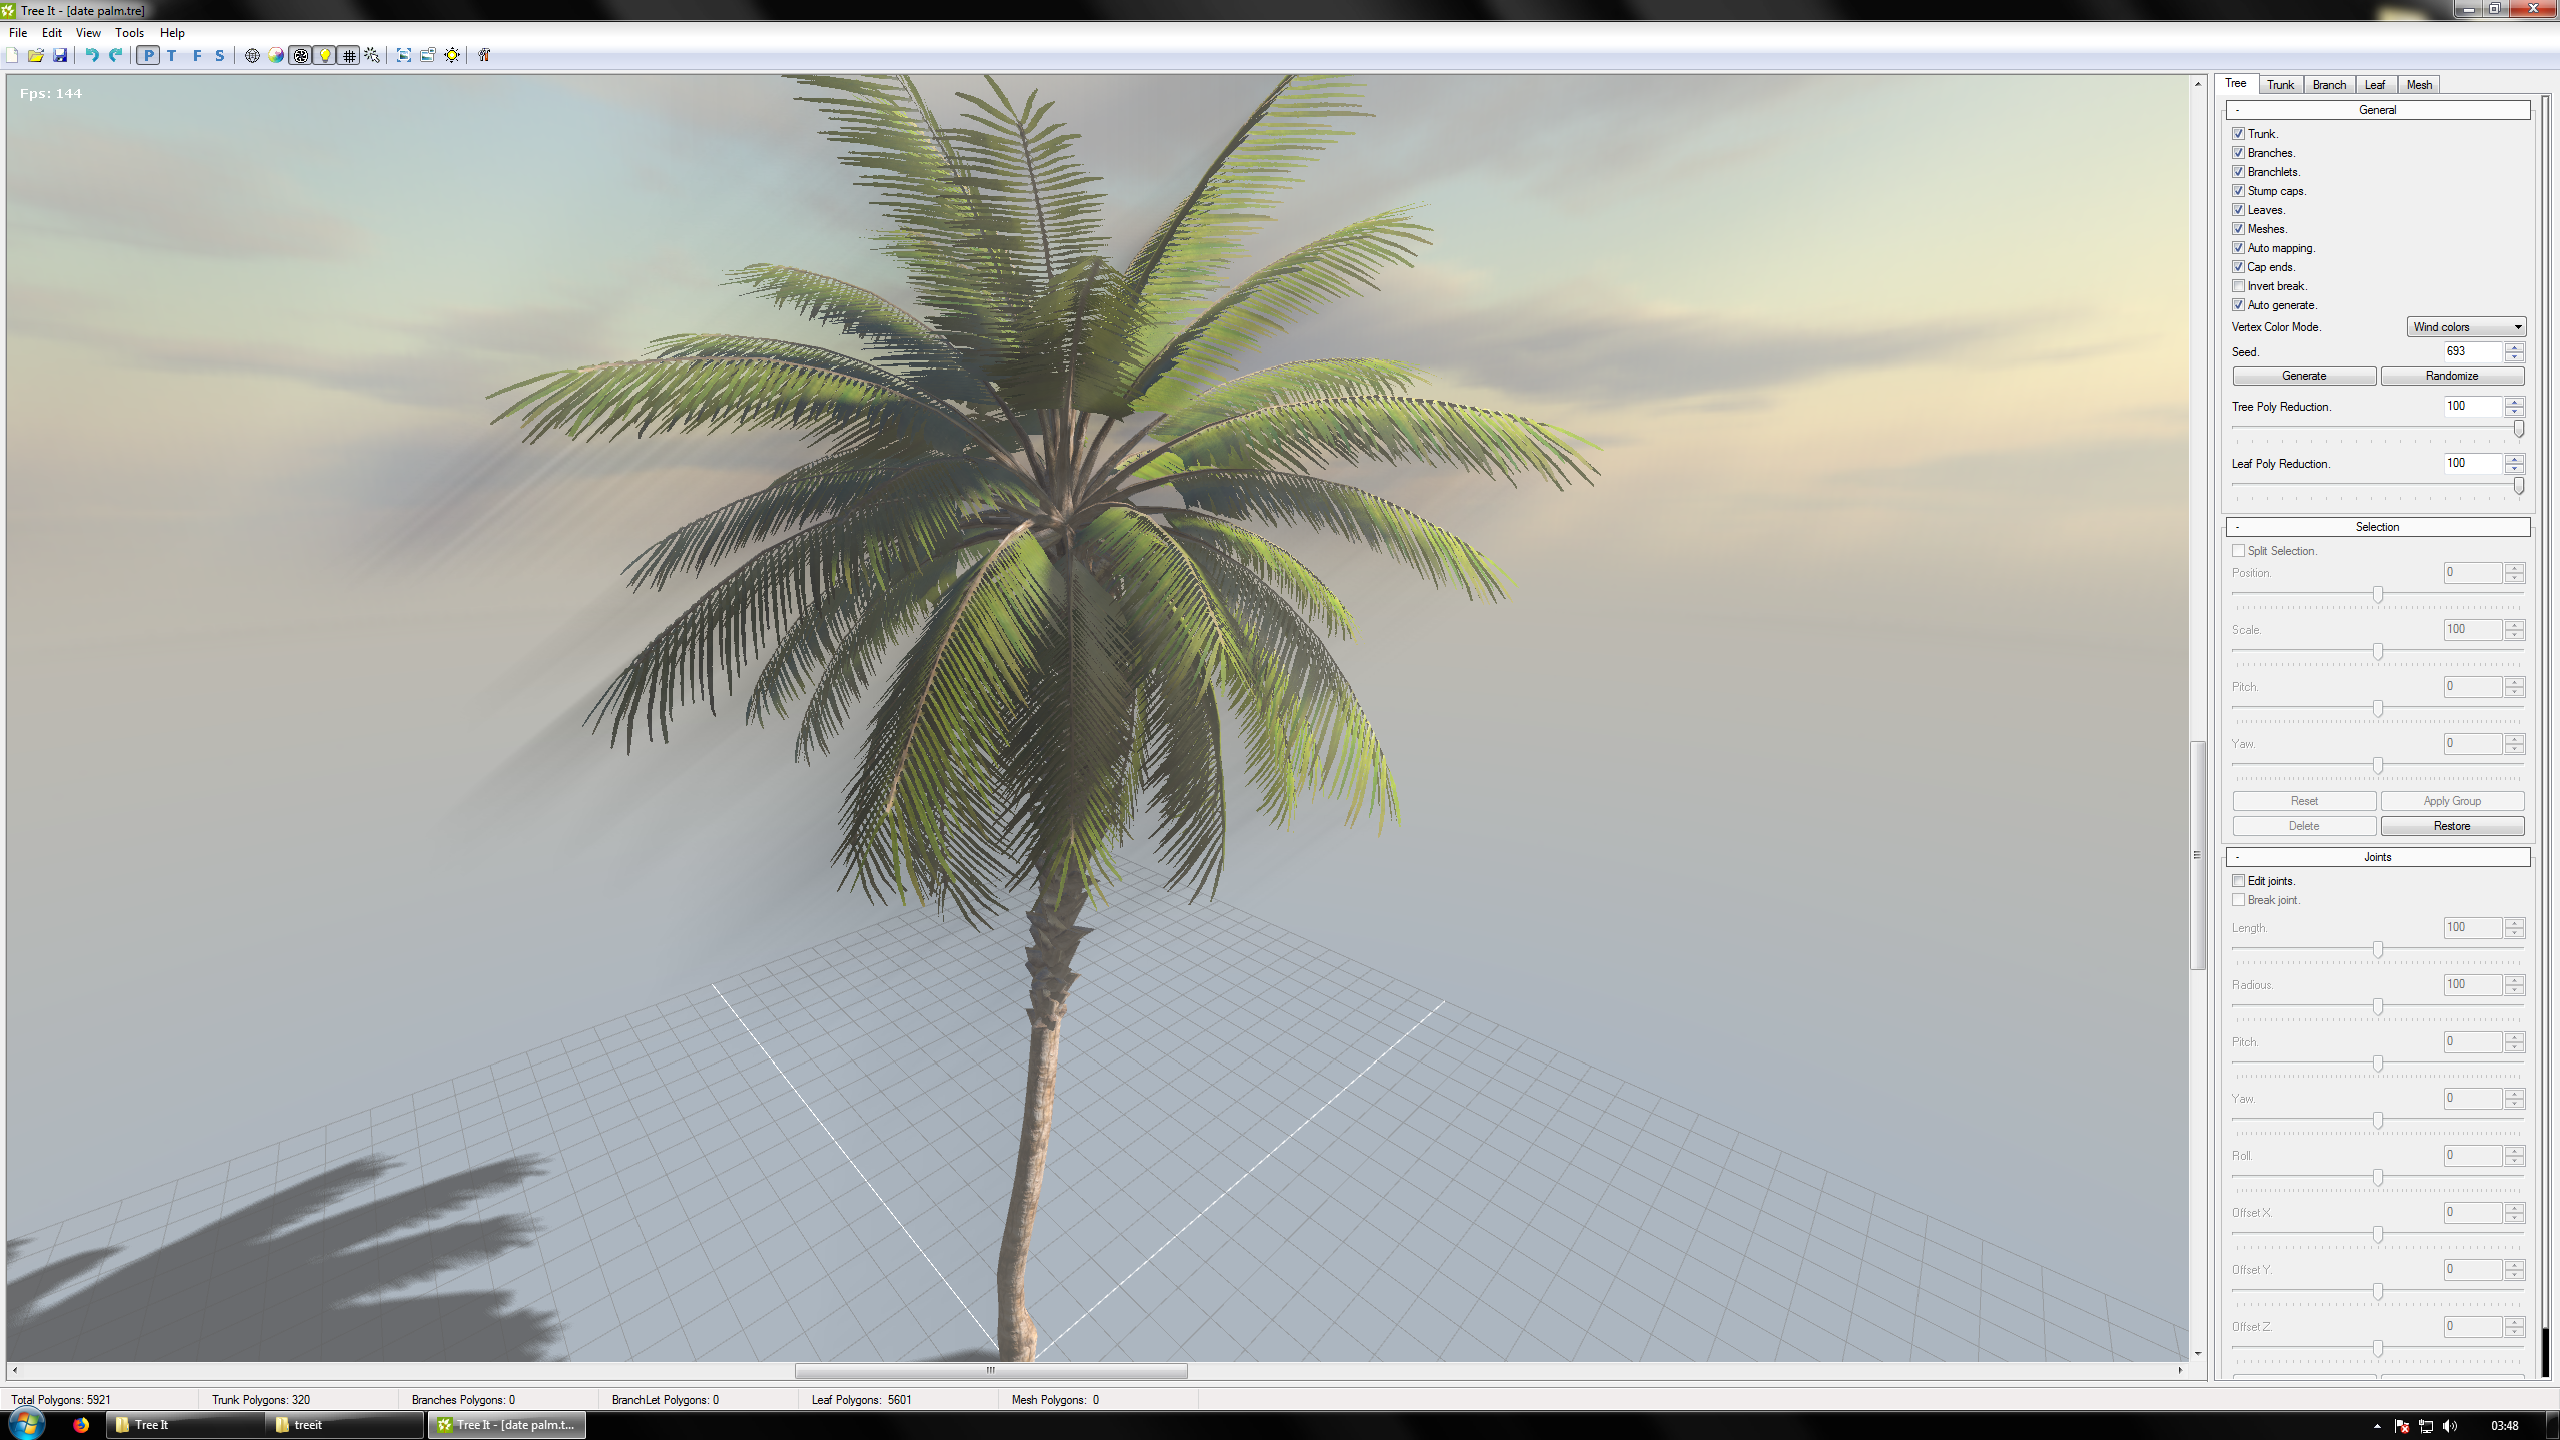
\includegraphics[width=0.8\textwidth]{treeit}
    \caption{Пример дерева, сгенерированного при помощи TreeIt.}
    \label{fig:treeit}
\end{figure}

\newpage
\section{TreeGen}
\emph{TreeGen} - плагин для генерации деревьев в редакторе трёхмерных моделей Blender, распространяемый свободно по лицензии MIT.

TreeGen использует комбинацию из двух подходов: системы Линденмайера и параметрический подход. Поддерживается очень большое количество различных параметров, позволяющих тонко настроить форму и распределение ветвей. TreeGen поддерживает генерацию листьев и цветков различной формы. Пример дерева, сгенерированного этим плагином, представлен на рисунке ~\ref{fig:treegen}.

\begin{figure}[h]
    \centering
    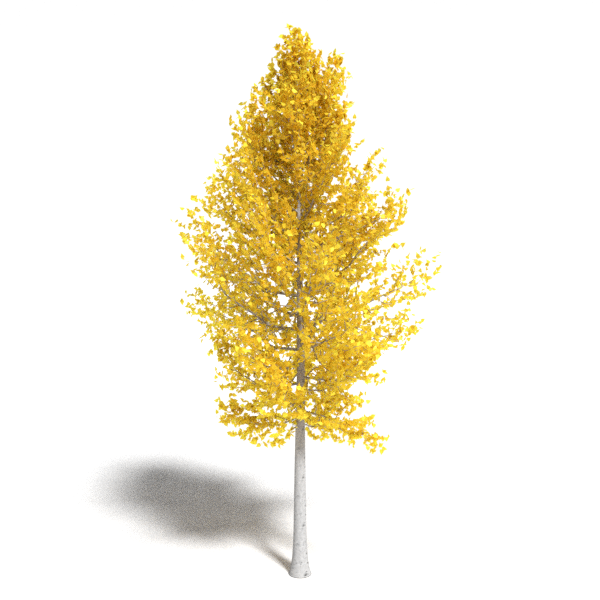
\includegraphics[width=0.8\textwidth]{treegen}
    \caption{Пример дерева, сгенерированного в плагине TreeGen.}
    \label{fig:treegen}
\end{figure}

\section{Unity Tree Creator}
В игровом движке Unity существует инструмент \emph{Tree Creator}, позволяющий создавать модели деревьев прямо в редакторе. Иерархия дерева представлена в виде графа, где вершины соответствуют группам ветвей или листьев. У каждого элемента этой иерархии есть отдельный набор параметров, включая начальное значение для генератора псеводслучайных чисел, распределение и уровень детализации. Пример созданного при помощи инструмента дерева приведён на рисунке ~\ref{fig:treeCreator}.

В редакторе есть возможность вручную перемещать контрольные точки ствола и ветвей, а также двигать листья. Кроме того, имеется встроенная поддержка анимаций ветра. Кнопка ``Create Wind Zone'' создаёт так называемую зону ветра, которая симулирует раскачивание деревьев на ветру в своей области действия. 

\begin{figure}[h]
    \centering
    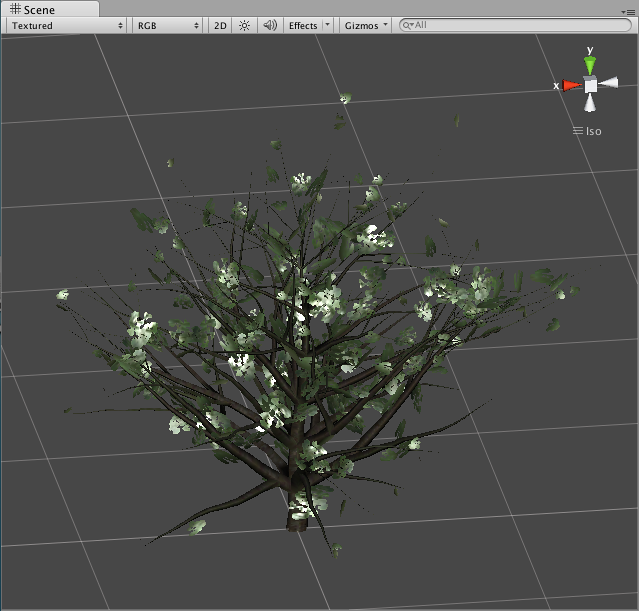
\includegraphics[width=0.8\textwidth]{treeCreator}
    \caption{Пример дерева, созданного с помощью инструмента Tree Creator.}
    \label{fig:treeCreator}
\end{figure}

Деревья, создаваемые с помощью этого инструмента, являются обычными игровыми объектами Unity и их параметры могут быть изменены во время выполнения. Теоретически, Tree Creator может быть использован для процедурной генерации моделей в самой игре путём программного изменения этих параметров. Однако данный инструмент предназначен для создания деревьев в редакторе и имеет очень большое количество параметров. Деревья создаются методом проб и ошибок, и поэтому генерировать качественные модели без использования редактора практически невозможно. 

\section{Заключение}
Большинство из рассмотренных аналоги генерируют модели деревьев с использованием L-систем, позволяя экспортировать их в файл и впоследствии использовать в каких-либо проектах. 

SpeedTree позволяет создавать высококачественные и реалистичные модели, оптимизированные для рендеринга в реальном времени. Тем не менее, алгоритмы, используемые этой системой, очень сложны и не подходят для генерации моделей в реальном времени. Другим важным недостатком является стоимость лицензии, которая может быть слишком высокой для независимых студий.

TreeIt бесплатен для использования и поддерживает множество форматов для экспорта. Также этот редактор очень прост в использовании и поддерживает генерацию растений. Однако это не кроссплатформенное приложение, в отличие от других рассмотренных аналогов. Более того, TreeIt не может использоваться для генерации моделей в реальном времени.

TreeGen имеет гибкие настройки генерации деревьев. Поскольку это плагин для Blender, сгенерированные деревья можно поместить в сцены, созданные в этом редакторе, или же перевести в полигональную сетку и отредактировать обычными средствами Blender. К тому же TreeGen является свободным программным обеспечением и его исходный код доступен на Github\cite{friggog}.

Unity Tree Creator, теоретически, может создавать модели деревьев во время выполнения программы, но не рассчитан на такое применение.  

В отличие от рассмотренных аналогов, разработанный в ходе выполнения данной работы плагин генерирует трёхмерные модели во время выполнения и подходит для использования в процедурно генерируемых уровней, в том числе в играх для мобильных платформ в силу низкого числа используемых полигонов.
\newpage
